\documentclass[border=10pt]{standalone}

\usepackage{tikz}
\usepackage{tikzsymbols}
\usetikzlibrary{calc,patterns,shapes.geometric}

\def\centerarc[#1](#2)(#3:#4:#5){\draw[#1] ($(#2)+({#5*cos(#3)},{#5*sin(#3)})$) arc (#3:#4:#5);}

\begin{document}
	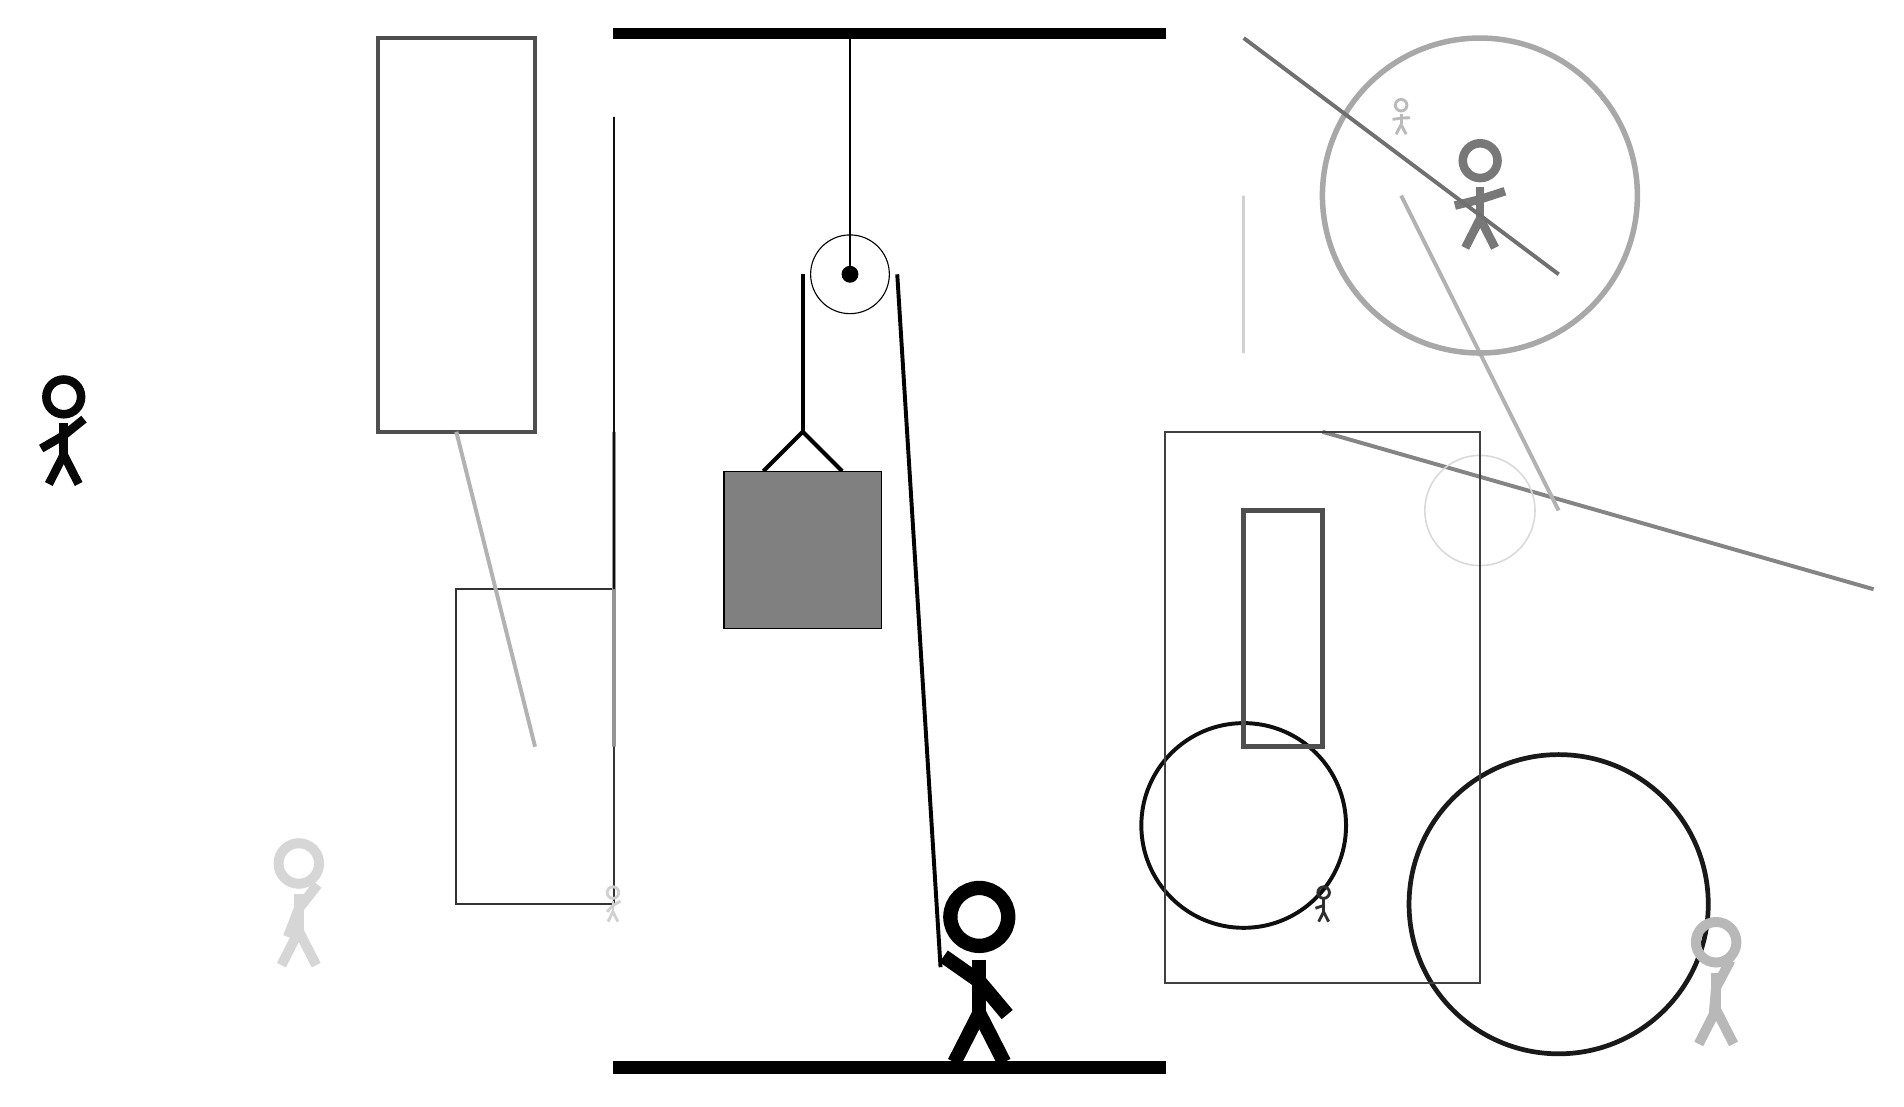
\begin{tikzpicture}
		%%%%% START %%%%%
		
		\draw[fill=black] (-2, 10) rectangle (5, 10.125);
		
		\draw (1, 7) circle (0.5);
		\draw[fill=black] (1, 7) circle (0.1);
		\draw (1, 10) -- (1, 7);
		
		\draw[line width=0.5mm] (-0.1, 4.5) -- (0.4, 5.0) -- (0.9, 4.5);
		\draw[fill=black!50] (-0.6, 4.5) rectangle (1.4, 2.5);
		
		\draw[line width=0.5mm] (0.4, 7) -- (0.4, 5.0);
		\centerarc[line width=0.5mm](1, 7)(0:180:0.6);
		\draw[line width=0.5mm](1.6, 7) -- (2.15, -1.8);
		
		\draw[line width=0.5mm, color=black!48](7, 5) -- (14, 3);
		
		\node[line width=0.4mm, color=black!53] at (9, 8) {\Strichmaxerl[6][14][18]};
		\draw[line width=0.3mm, color=black!80] (-2, 3) rectangle (-4, -1);
		\node[line width=0.7mm, color=black!27] at (8, 9) {\Strichmaxerl[2][9][2]};
		\draw[line width=0.5mm, color=black!30](10, 4) -- (8, 8);
		\node[line width=0.2mm, color=black!18] at (-2, -1) {\Strichmaxerl[2][47][30]};
		\node[line width=0.5mm, color=black!97] at (-9, 5) {\Strichmaxerl[6][30][39]};
		\draw[line width=0.5mm, color=black!42] (-2, 5) rectangle (-2, 1);
		\draw [line width=0.6mm, color=black!90](10, -1) circle (1.9);
		\draw[line width=0.5mm, color=black!69] (-3, 10) rectangle (-5, 5);
		\draw [line width=0.7mm, color=black!34](9, 8) circle (2.0);
		\draw [line width=0.5mm, color=black!94](6, 0) circle (1.3);
		\draw[line width=0.5mm, color=black!56](6, 10) -- (10, 7);
		\draw[line width=0.3mm, color=black!94] (-2, 9) rectangle (-2, 3);
		\draw [line width=0.2mm, color=black!15](9, 4) circle (0.7);
		\node[line width=0.5mm, color=black!28] at (12, -2) {\Strichmaxerl[7][85][62]};
		
		\node[line width=0.7mm, color=black!16] at (-6, -1) {\Strichmaxerl[7][69][52]};
		
		\draw[line width=0.3mm, color=black!75] (5, 5) rectangle (9, -2);
		\draw[line width=0.6mm, color=black!69] (6, 1) rectangle (7, 4);
		
		\draw[line width=0.5mm, color=black!30](-4, 5) -- (-3, 1);
		\node[line width=0.7mm, color=black!82] at (7, -1) {\Strichmaxerl[2][19][90]};
		
		\draw[line width=0.4mm, color=black!18] (6, 8) rectangle (6, 6);
		
		\node at (2.6, -1.9) {\Strichmaxerl[10][-35][-50]};
		
		\draw[fill=black] (-2, -3) rectangle (5, -3.15);
		
		%%%%% END %%%%%
	\end{tikzpicture}
\end{document}